\documentclass{article}

\usepackage[letterpaper, top=1in, bottom=1in, left=1in, right=1in]{geometry}
\usepackage{
    physics, 
    amsmath, 
    enumitem, 
    nicefrac, 
    fancyhdr, 
    microtype, 
    pgfplots, 
    tikz, 
    float,
    hyperref
}

\pgfplotsset{compat=newest}
\pagestyle{fancy}

\title{Friction and Circular Motion}
\author{Laith Toom}
\date{21/2/2023}

\begin{document}
\maketitle
\newpage

\section{Friction}
When a object is moving along a surface, there is a force acting 
against that movement, and that force is friction $\va{f}$.

\begin{figure}[h]
    \centering
    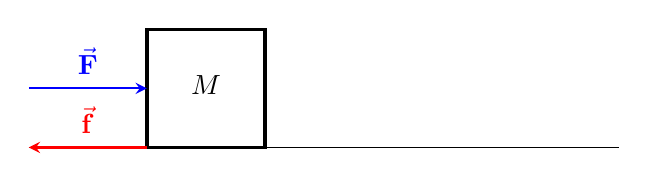
\begin{tikzpicture}[scale=1.5]
        \draw (0, 0) -- (5, 0);

        \draw[very thick] (1, 0) -- (1, 1) -- (2, 1) node[midway, yshift=-20] {$M$} -- (2, 0) --(1, 0);

        \draw[thick, -stealth, blue] (0, 0.5) -- (1, 0.5) node[midway, yshift=10] {$\va{F}$};
        \draw[thick, -stealth, red] (1, 0) -- (0, 0) node[midway, yshift=10] {$\va{f}$};
    \end{tikzpicture}
    \caption{Box moving along ground with friction $\va{f}$}
\end{figure}

The relationship between $\va{f}$ and $\va{F}$ is linear with a slope of 1, meaning that
there is a 1:1 ratio between friction and the force moving the box. As a result, the two 
forces cancel out and no movement occurs. 

However, this only holds true until friction reaches its maximum force:
\begin{figure}[h]
    \centering 
    \vspace{-1em}
    \caption{$\va{f}$ with respect to $\va{F}$}
    \vspace{0.8em}
    \begin{tikzpicture}
        \begin{axis}
        [
            ymax=5, ymin=0,
            xmax=10, xmin=0,
            xlabel = $\va{F}$,
            ylabel = $\va{f}$,
            % title = $\va{f}$ with respect to $\va{F}$,
            legend pos = outer north east,
        ]
        \plot[no marks, domain={0:3}, color=red] {x};
        \addlegendentry{No movement}
        \plot[no marks, domain={3:10}, color=blue] {3};
        \addlegendentry{Movement}
        \end{axis}
    \end{tikzpicture}
\end{figure}

The maximum force of friction, $\va{f}_\mathrm{max}$, is defined as the product of 
the \textbf{coefficient of friction}, $\mu$, and the normal force, $\va{N}$, acting on 
the object:
\[ \va{f}_\mathrm{max} = \mu\va{N} \]
$\mu$ will be a given constant, and it depends on the type of surface where movement is
occuring. Slippery surfaces such as ice will have a lower coefficient while rought 
surfaces such as asphalt or concrete will have a higher coefficient.

\newpage
\section{Cricular Motion}
Does a object in circular motion with a constant speed have a force acting on it?
\begin{figure}[h]
    \centering
    \label{fig:3}
    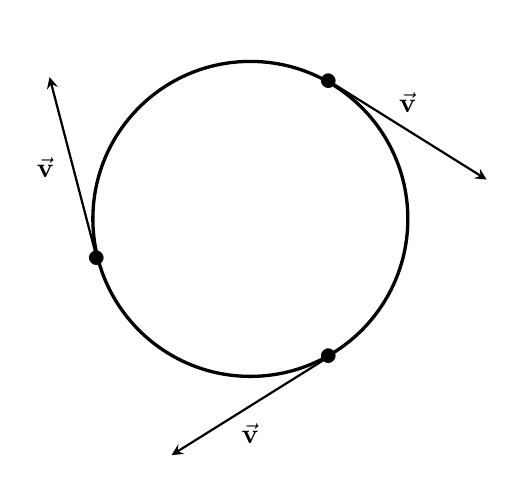
\begin{tikzpicture}
        \draw[very thick] (0, 0) arc (0:360:2); 

        \draw[thick, -stealth] (-1, 1.75) node[scale=5] {.} -- (1, 0.5) node[midway, yshift=10] {$\va{v}$};
        \draw[thick, -stealth] (-1, -1.75) node[scale=5] {.} -- (-3, -3) node[midway, yshift=-10] {$\va{v}$};
        \draw[thick, -stealth] (-3.95, -0.5) node[scale=5] {.} -- (-4.55, 1.8) node[midway, xshift=-10] {$\va{v}$};
    \end{tikzpicture}
    \caption{Velocity of object in circular motion}
\end{figure}

\noindent An object in circular motion does have a force acting on it because 
the direction of velocity changes, which means the componenets of velocity change,
and for there to be change in velocity, there must be acceleration. 

However, the magnitude of velocity, \textbf{speed}, in this scenario is costant, 
it is only the componenets that are changing:
\begin{align*}
    &\abs{\va{v}} = \sqrt{{v_x}^2 + {v_y}^2} \\
    &\derivative{\abs{\va{v}}}{t} = 0 \\
    &\derivative{v_x}{t} = a_x \\
    &\derivative{v_y}{t} = a_y
\end{align*}
if you forgot, acceleration $\va{a}$ is also a vector, with $x$ and $y$ componenets acting 
on the respective $x$ and $y$ componenets of velocity $\va{v}$.

\subsection{Determing the Componenets of Velocity}
We can redraw \hyperref[fig:3]{Figure 3} with axes $x$ and $y$:
\begin{figure}[H]
    \centering
    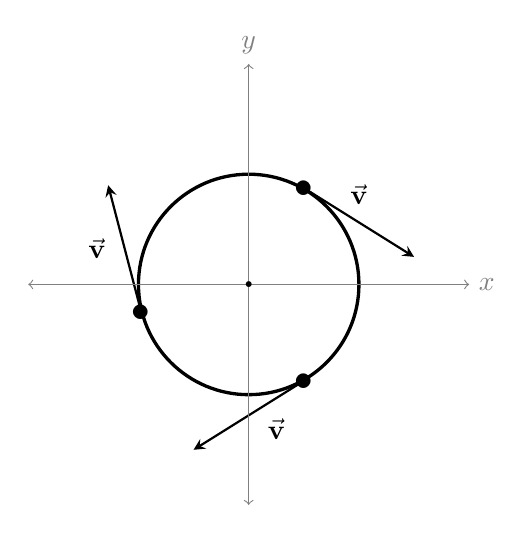
\begin{tikzpicture}[scale=0.7]
        \draw[very thick] (0, 0) arc (0:360:2); 

        \draw[thick, -stealth] (-1, 1.75) node[scale=5] {.} -- (1, 0.5) node[midway, yshift=10] {$\va{v}$};
        \draw[thick, -stealth] (-1, -1.75) node[scale=5] {.} -- (-3, -3) node[midway, yshift=-5, xshift=10] {$\va{v}$};
        \draw[thick, -stealth] (-3.95, -0.5) node[scale=5] {.} -- (-4.55, 1.8) node[midway, xshift=-10] {$\va{v}$};

        \draw[<->, gray] (-2, -4) -- (-2, 4) node[above] {$y$};
        \draw[<->, gray] (-6, 0) -- (2, 0) node[right] {$x$};
        \node[scale=2] at (-2, 0) {.};
    \end{tikzpicture}
\end{figure}

We can also draw displacement vectors $\va{r}$ from the origin to the start of the 
velocity vectors:
\begin{figure}[H]
    \centering
    \begin{tikzpicture}[scale=1]
        \draw[very thick] (0, 0) arc (0:360:2); 

        \draw[thick, -stealth] (-1, 1.75) node[scale=4] (v1) {.} -- (1, 0.5) node[midway, yshift=10] {$\va{v}$};
        \draw[thick, -stealth] (-1, -1.75) node[scale=4] (v2) {.} -- (-3, -3) node[midway, yshift=-5, xshift=10] {$\va{v}$};
        \draw[thick, -stealth] (-3.95, -0.5) node[scale=4] (v3) {.} -- (-4.55, 1.8) node[midway, xshift=-10] {$\va{v}$};

        \draw[<->, gray] (-2, -4) -- (-2, 4) node[above] {$y$};
        \draw[<->, gray] (-6, 0) -- (2, 0) node[right] {$x$};
        \node[scale=2] at (-2, 0) {.};

        \draw[-stealth] (-2, 0) -- (-1.05, 1.65) node[midway, xshift=-5, yshift=2] {$\va{r}$};
        \draw[-stealth] (-2, 0) -- (-1.05, -1.65) node[midway, xshift=-6, yshift=-2] {$\va{r}$};
        \draw[-stealth] (-2, 0) -- (-3.85, -0.48) node[midway, xshift=0, yshift=-5] {$\va{r}$};
    \end{tikzpicture}
\end{figure}

Decomposing the displacement vectors into $r_x$ and $r_y$ will form triangles, which will allow
us to solve for those componenets of displacement:
\begin{align*}
    r_x &= r\cos(\theta) \\
    r_y &= r\sin(\theta)
\end{align*}
we can then differeniate to get the componenets of velocity:
\begin{align*}
    v_x &= \derivative{r_x}{t} = -r\sin(\theta) \derivative{\theta}{t} \\[1ex]
    v_y &= \derivative{r_y}{t} = r\cos(\theta) \derivative{\theta}{t} \\
\end{align*}
if you can visualize it, as the object moves around the circle, the displacement vector
$\va{r}$ follows it, and so componenets of the displacement vector change. Thus, a new 
triangle is formed, which means a new value for $\theta$, thus $\theta$ does have a rate 
of change, which comes out during differentiation as seen above.

The rate of change of $\theta$ will be represented as omega $\omega$:
\[ \omega = \derivative{\theta}{t} \]

\end{document}